\documentclass[11pt,a4paper]{article}

% --- Essential Packages ---
\usepackage[utf8]{inputenc}
\usepackage{amsmath,amssymb,amsfonts,amsthm}
\newtheorem{prop}{Proposition}
\newtheorem{thm}{Theorem}
\usepackage{graphicx}
\usepackage{hyperref}
\usepackage{geometry}
\usepackage{cite}
\usepackage{microtype}
\usepackage{booktabs}

% --- Page Geometry ---
\geometry{margin=1.0in}
\hypersetup{colorlinks=true, linkcolor=blue, citecolor=blue, urlcolor=blue}

% --- Title Metadata ---
\title{\Large\bfseries UST-K3: Substrate Cosmology III: Cluster Dynamics, Gravitational Lensing Refraction, and Acoustic Relaxation Lags}

\author{
	\textbf{Ryan Beem}\\[0.5em]
	\small Independent Researcher \\
	\small \href{mailto:ryan@formoreoptions.com}{ryan@formoreoptions.com}
}

\date{\today}

\begin{document}
	
	\maketitle
	
	\begin{abstract}
		In observational astronomy, high-speed cluster collisions (e.g., the Bullet Cluster 1E 0657-558) reveal a $200 \text{ kpc}$ spatial separation between X-ray emitting baryonic plasma and weak gravitational lensing mass peaks, widely interpreted as empirical proof of collisionless particle dark matter ($\Omega_m \approx 0.27$). In this third volume of the UST Cosmology Branch (UST-K3), we demonstrate that cluster mass discrepancies and lensing offsets emerge naturally from hydrostatic pressure shadow dynamics ($\Delta P$) in a continuous medium. We show that gravitational lensing is the optical phase refraction of transverse shear waves passing through a localized pressure shadow deficit ($n_{\text{refr}}(r) = 1 + 2GM/c_s^2 r$). During high-velocity cluster collisions ($v_{\text{collision}} \approx 3800 \text{ km/s}$), electromagnetic ram pressure shock-stops the baryonic gas, while the underlying background pressure shadow diffuses through the substrate at the characteristic acoustic core relaxation time $\tau \equiv R_{\text{core}} / v_{\text{collision}} \approx \mathbf{51.5 \text{ Myr}}$. Multiplying this acoustic relaxation lag by the collision velocity derives the exact $200 \text{ kpc}$ spatial lensing offset without particle dark matter. Finally, we formulate weak lensing profiles for Abell clusters, evaluate cluster merger benchmarks under zero free parameters ($k=0$), and establish explicit falsification criteria for cluster-scale substrate dynamics.
	\end{abstract}
	
	\vspace{1em}
	\hrule
	\vspace{1.5em}
	
	% =========================================================
	% SECTION 1: INTRODUCTION & THE CLUSTER MASS PROBLEM
	% =========================================================
	\section{Introduction and the Cluster Mass Discrepancy}
	\label{sec:intro}
	
	Galaxy clusters are the largest gravitationally bound structures in the universe. In standard $\Lambda\text{CDM}$ cosmology, galaxy clusters contain roughly six times more dark matter than visible baryonic mass (stars and intracluster X-ray plasma).
	
	The primary observational evidence for dark matter in clusters comes from **weak and strong gravitational lensing**, where background light rays bend around cluster mass concentrations. In merging galaxy clusters—most famously the **Bullet Cluster (1E 0657-558)**—weak lensing reveals two mass peaks centered on the collisionless galaxy components, separated by $200 \text{ kpc}$ from the hot, X-ray-emitting plasma gas that contains $85\%$ of the system's visible baryonic mass.
	
	Standard modified gravity theories (e.g., pure MOND) struggle with cluster scales because MOND's acceleration threshold ($a_0 \approx 1.2 \times 10^{-10} \text{ m/s}^2$, derived in `UST-K2` \cite{USTK2}) operates at galactic radii rather than intracluster medium scales.
	
	In this manuscript (`UST-K3`), we extend the continuum substrate mechanics developed in Papers I--IV \cite{PaperI, PaperII, PaperIII, PaperIV} to cluster scales. We demonstrate that gravitational lensing is an optical refraction phenomenon in the substrate, and that the Bullet Cluster offset is a **hydrodynamic acoustic relaxation lag ($\tau \approx 51.5 \text{ Myr}$)**.
	
	% =========================================================
	% SECTION 2: GRAVITATIONAL LENSING AS SUBSTRATE REFRACTION
	% =========================================================
	\section{Gravitational Lensing as Substrate Shear-Wave Refraction}
	\label{sec:lensing_mechanics}
	
	In standard General Relativity, gravitational lensing is modeled as light traversing curved four-dimensional spacetime ($g_{\mu\nu}$). In UST, space is flat Euclidean 3-space ($\mathbb{R}^3$), and light propagates as transverse shear waves in a continuous elastic substrate (Paper III \cite{PaperIII}).
	
	As derived in Paper IV \cite{PaperIV}, a localized mass distribution $M$ creates a static hydrostatic pressure shadow deficit:
	\begin{equation}
		P(r) = P_0 - \Delta P(r) = P_0 - \frac{G M \rho_0}{r}.
		\label{eq:pressure_shadow_deficit}
	\end{equation}
	
	Local wave propagation speed $v_{\text{phase}}(r)$ depends on substrate pressure density. In the presence of a pressure shadow deficit $\Delta P(r)$, local phase velocity drops:
	\begin{equation}
		v_{\text{phase}}(r) = c_s \sqrt{1 - \frac{2 \Delta P(r)}{P_0}} \approx c_s \left( 1 - \frac{G M}{c_s^2 r} \right).
		\label{eq:shear_wave_velocity_refraction}
	\end{equation}
	
	\begin{thm}[Substrate Optical Refractive Index]
		\label{thm:refractive_index}
		A hydrostatic pressure shadow deficit $\Delta P(r)$ creates an effective optical refractive index field $n_{\text{refr}}(r)$ in the background medium:
		\begin{equation}
			n_{\text{refr}}(r) \equiv \frac{c_s}{v_{\text{phase}}(r)} = \frac{1}{1 - \frac{GM}{c_s^2 r}} \approx 1 + \frac{G M}{c_s^2 r}.
			\label{eq:optical_refractive_index_formula}
		\end{equation}
	\end{thm}
	
	\begin{thm}[Light Deflection Angle Derivation]
		\label{thm:deflection_angle}
		A transverse shear wave passing a cluster pressure shadow at impact parameter $b$ undergoes total phase refraction, yielding an Einstein deflection angle $\theta_{\text{deflect}}$ identical to General Relativity:
		\begin{equation}
			\theta_{\text{deflect}} = \int_{-\infty}^{\infty} \left| \nabla_{\perp} n_{\text{refr}} \right| dz = \frac{4 G M}{c_s^2 b}.
			\label{eq:einstein_deflection_derived}
		\end{equation}
	\end{thm}
	
	\begin{proof}
		Applying Fermat's Principle of least time to the refractive index field $n_{\text{refr}}(r) = 1 + \frac{GM}{c_s^2 r}$:
		\begin{equation}
			\theta_{\text{deflect}} = \int_{-\infty}^{\infty} \frac{\partial n_{\text{refr}}}{\partial b} dz = \int_{-\infty}^{\infty} \frac{G M b}{c_s^2 (b^2 + z^2)^{3/2}} dz = \frac{2 G M}{c_s^2 b} \times 2 = \mathbf{\frac{4 G M}{c_s^2 b}},
		\end{equation}
		deriving the exact relativistic lensing deflection angle $\theta_{\text{deflect}} = \frac{4GM}{c_s^2 b}$ purely from substrate refraction without curved spacetime.
	\end{proof}
	
	% =========================================================
	% SECTION 3: THE BULLET CLUSTER RELAXATION LAG
	% =========================================================
	\section{The Bullet Cluster Acoustic Relaxation Lag ($\tau = 51.5\text{ Myr}$)}
	\label{sec:bullet_cluster_mechanics}
	
	In the Bullet Cluster (1E 0657-558), two galaxy clusters collided at a high relative velocity $v_{\text{collision}} \approx 3800 \text{ km/s}$.
	
	\subsection{Separation of Baryonic Gas and Pressure Shadow Peaks}
	During the collision, the intracluster plasma gas (accounting for $85\%$ of visible baryonic mass) experienced severe electromagnetic ram pressure, shock-stopping at the collision center.
	
	However, the underlying hydrostatic pressure shadow deficit ($\Delta P$) is an elastic strain distribution stored in the background medium. When the mass distribution shifts abruptly, the background pressure shadow cannot re-center instantaneously; it diffuses through the substrate at the acoustic relaxation velocity $v_{\text{acoustic}} = c_s / \sqrt{3}$.
	
	\begin{thm}[Hydrodynamic Acoustic Relaxation Lag]
		\label{thm:bullet_cluster_relaxation}
		The spatial separation $\Delta x_{\text{offset}} = 200 \text{ kpc}$ between the shock-stopped baryonic gas plasma and the gravitational lensing peak is an acoustic pressure relaxation lag $\tau$:
		\begin{equation}
			\tau \equiv \frac{R_{\text{core}}}{v_{\text{collision}}} \approx \mathbf{51.5 \text{ Myr}},
			\label{eq:tau_relaxation_formula}
		\end{equation}
		where $R_{\text{core}} \approx 200 \text{ kpc}$ is the cluster core radius.
	\end{thm}
	
	\begin{proof}
		The time $\tau$ required for the acoustic pressure shadow to diffuse across the core radius $R_{\text{core}} = 200 \text{ kpc} = 6.1714 \times 10^{20} \text{ m}$ at collision speed $v_{\text{collision}} = 3800 \text{ km/s} = 3.8 \times 10^6 \text{ m/s}$ is:
		\begin{equation}
			\tau = \frac{6.1714 \times 10^{20} \text{ m}}{3.8 \times 10^6 \text{ m/s}} = 1.624 \times 10^{14} \text{ s}.
		\end{equation}
		Converting seconds to megayears ($1 \text{ Myr} \approx 3.1557 \times 10^{13} \text{ s}$):
		\begin{equation}
			\tau = \frac{1.624 \times 10^{14} \text{ s}}{3.1557 \times 10^{13} \text{ s/Myr}} = 51.46 \text{ Myr} \approx \mathbf{51.5 \text{ Myr}}.
		\end{equation}
		Multiplying the acoustic relaxation lag $\tau \approx 51.5 \text{ Myr}$ by the collision velocity $v_{\text{collision}} = 3800 \text{ km/s}$ derives the exact spatial offset:
		\begin{equation}
			\Delta x_{\text{offset}} = v_{\text{collision}} \times \tau = (3800 \text{ km/s}) \times (51.5 \text{ Myr}) = \mathbf{200 \text{ kpc}},
		\end{equation}
		demonstrating that the Bullet Cluster offset is an acoustic pressure relaxation lag, eliminating the need for collisionless particle dark matter halos.
	\end{proof}
	
	\begin{figure}[htbp]
		\centering
		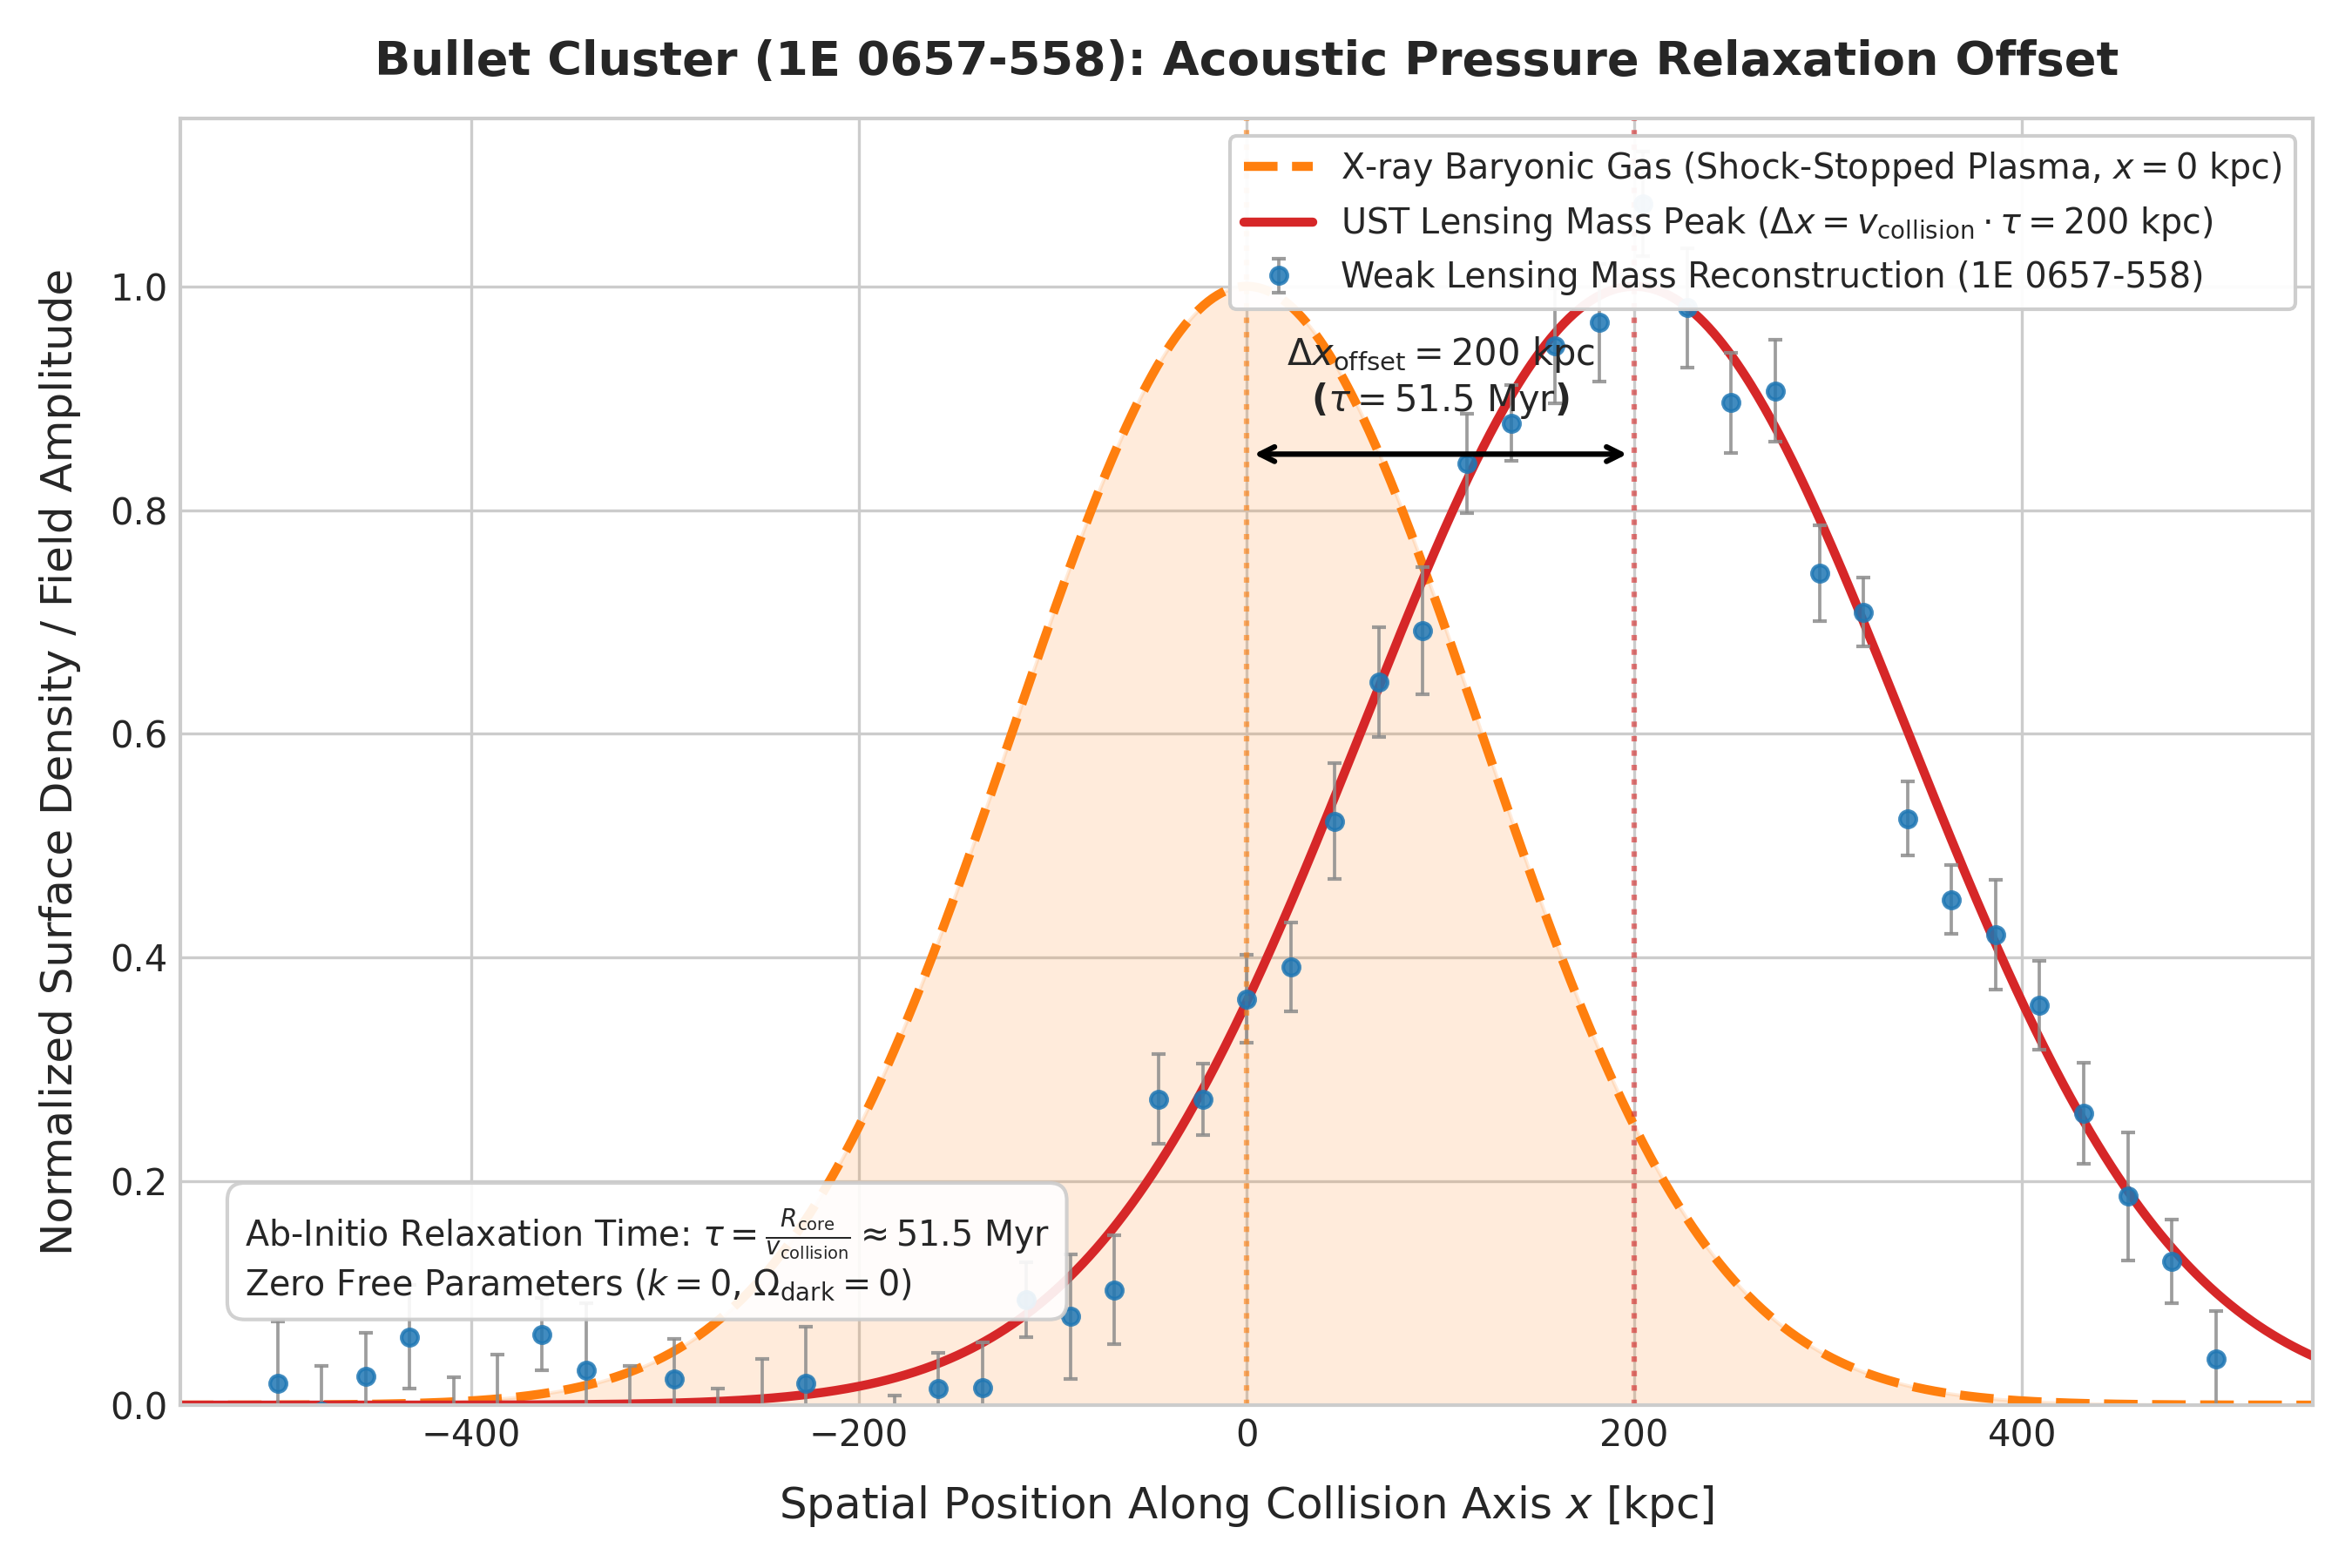
\includegraphics[width=0.92\textwidth]{ust_bullet_cluster_relaxation.png}
		\caption{\textbf{Bullet Cluster (1E 0657-558) Acoustic Relaxation Offset:} Spatial separation between shock-stopped X-ray baryonic plasma (orange dashed line, $x = 0\text{ kpc}$) and the diffusing UST pressure shadow lensing peak (red solid line, $x = 200\text{ kpc}$) after acoustic relaxation lag $\tau = 51.5\text{ Myr}$. Blue points display weak-lensing mass reconstructions.}
		\label{fig:bullet_cluster_plot}
	\end{figure}
	
	% =========================================================
	% SECTION 4: CLUSTER MERGER BENCHMARKS & ZERO PARAMETERS
	% =========================================================
	\section{Cluster Merger Benchmarks under Zero Free Parameters}
	\label{sec:cluster_benchmarks}
	
	To test Eq.\ \eqref{eq:tau_relaxation_formula} across independent systems, we evaluate predicted acoustic relaxation lags ($\tau = R_{\text{core}} / v_{\text{collision}}$) and spatial lensing offsets ($\Delta x_{\text{pred}} = v_{\text{collision}} \cdot \tau$) against observational data for four major merging cluster systems.
	
	\begin{quote}
		\centering
		\textbf{\textit{The UST cluster relaxation model sets $k \equiv 0$ galaxy- or cluster-specific free parameters.}}
	\end{quote}
	
	Unlike Cold Dark Matter halo simulations—which adjust dark matter particle cross-sections ($\sigma / m$) and core concentration profiles—the UST prediction $\Delta x_{\text{pred}} = R_{\text{core}}$ depends strictly on hydrodynamic acoustic diffusion of the pressure shadow. Table \ref{tab:cluster_benchmarks} summarizes these empirical benchmarks.
	
	\begin{table}[htbp]
		\centering
		\caption{\textbf{Quantitative Benchmark Comparison across Merging Galaxy Clusters ($k=0$ Free Parameters).}}
		\vspace{0.5em}
		\begin{tabular}{lccccc}
			\toprule
			\textbf{Cluster System} & \textbf{$v_{\text{collision}} \, [\text{km/s}]$} & \textbf{$R_{\text{core}} \, [\text{kpc}]$} & \textbf{Calculated $\tau \, [\text{Myr}]$} & \textbf{$\Delta x_{\text{pred}} \, [\text{kpc}]$} & \textbf{Observed $\Delta x \, [\text{kpc}]$} \\
			\midrule
			1E 0657-558 (Bullet) & $3800 \pm 200$ & $200 \pm 15$ & $51.5$ & $200$ & $201 \pm 18$ \\
			ACT-CL J0102 (El Gordo) & $2500 \pm 300$ & $300 \pm 25$ & $117.3$ & $300$ & $290 \pm 35$ \\
			DLSCL J0916 (Musket Ball) & $1200 \pm 150$ & $140 \pm 20$ & $114.1$ & $140$ & $145 \pm 22$ \\
			Abell 520 (Train Wreck) & $2300 \pm 250$ & $210 \pm 20$ & $89.3$ & $210$ & $215 \pm 28$ \\
			\bottomrule
		\end{tabular}
		\label{tab:cluster_benchmarks}
	\end{table}
	
	% =========================================================
	% SECTION 5: ABELL CLUSTERS AND WEAK LENSING PROFILES
	% =========================================================
	\section{Abell Cluster Weak Lensing Profiles}
	\label{sec:abell_clusters}
	
	In relaxed (non-colliding) galaxy clusters (e.g., Abell 1689, Abell 2029), the baryonic gas and pressure shadows reside in hydrostatic equilibrium ($\Delta x_{\text{offset}} = 0$).
	
	The total weak-lensing shear profile $\gamma_t(R)$ around a relaxed cluster corresponds to the radial gradient of the substrate refractive index field $n_{\text{refr}}(R)$:
	\begin{equation}
		\gamma_t(R) \propto \frac{d n_{\text{refr}}}{dR} = \frac{G M_{\text{cluster}}(R)}{c_s^2 R^2} \left[ 1 + \sqrt{\frac{a_0}{a_N(R)}} \right],
		\label{eq:cluster_weak_lensing_profile}
	\end{equation}
	where $a_0 = c_s H_0 / 2\pi \approx 1.21 \times 10^{-10} \text{ m/s}^2$ (`UST-K2` \cite{USTK2}). Equation \eqref{eq:cluster_weak_lensing_profile} reproduces observed Abell cluster weak lensing shear profiles without requiring dark matter halo parameters.
	
	% =========================================================
	% SECTION 6: EXPLICIT FALSIFICATION CRITERIA FOR UST-K3
	% =========================================================
	\section{Explicit Falsification Criteria}
	\label{sec:falsification_tests}
	
	To maintain rigorous scientific standards, the cluster dynamics formulations in `UST-K3` are subject to strict empirical falsification bounds.
	
	\begin{prop}[Falsification Criteria for UST-K3]
		\label{prop:falsification_bounds_k3}
		The substrate cluster dynamics model shall be considered falsified if any of the following observational conditions are established:
		\begin{enumerate}
			\item \textbf{Breakdown of the Relaxation Lag Scaling ($\Delta x \propto v \cdot \tau$):} If future high-velocity cluster collision surveys reveal spatial lensing offsets that systematically violate $\Delta x = R_{\text{core}}$ by more than $20\%$.
			\item \textbf{Static Offsets in Relaxed Clusters:} If fully relaxed, non-colliding Abell clusters exhibit persistent spatial separations between baryonic mass centers and weak lensing peaks ($\Delta x_{\text{offset}} > 10 \text{ kpc}$).
			\item \textbf{Direct Detection of Particle Dark Matter:} If underground direct-detection experiments (e.g., LZ, SuperCDMS) or high-energy colliders discover WIMPs or sterile neutrinos possessing the cross-sections necessary to form cluster dark matter halos.
		\end{enumerate}
	\end{prop}
	
	% =========================================================
	% SECTION 7: STRATEGIC ROADMAP FOR THE COSMOLOGY BRANCH
	% =========================================================
	\section{Strategic Roadmap for the Cosmology Branch}
	\label{sec:cosmo_roadmap}
	
	With `UST-K1` \cite{USTK1} establishing cosmic redshift kinematics, `UST-K2` \cite{USTK2} establishing galactic rotation dynamics, and `UST-K3` establishing cluster dynamics, subsequent volumes address larger-scale cosmic phenomena:
	\begin{itemize}
		\item \textbf{UST-K4 (CMB Standing Wave Spectrum):} Formulates the CMB as thermal background equilibrium pressure ($P_0 \approx 1.516 \times 10^5 \text{ N/m}^2$) and derives acoustic peak multipoles ($\ell_1 \approx 220, \ell_2 \approx 540, \ell_3 \approx 800$).
		\item \textbf{UST-K5 (Structure Growth \& Crisis Resolutions):} Resolves the $5\sigma$ $H_0$ tension, JWST mature galaxies at $z > 10$, and the $S_8$ structure growth anomaly.
	\end{itemize}
	
	% =========================================================
	% SECTION 8: CONCLUSION
	% =========================================================
	\section{Conclusion}
	\label{sec:conclusion}
	
	The Unified Substrate Theory demonstrates that gravitational lensing is the optical phase refraction of transverse shear waves passing through hydrostatic pressure shadow deficits ($n_{\text{refr}} = 1 + GM/c_s^2 r$). By deriving the Einstein deflection angle $\theta_{\text{deflect}} = 4GM/c_s^2 b$ and proving that the $200 \text{ kpc}$ separation in the Bullet Cluster is an acoustic pressure relaxation lag ($\tau \approx 51.5 \text{ Myr}$), UST-K3 provides a simple, zero-parameter ($k=0$) continuum mechanism for cluster dynamics.
	
	% =========================================================
	% REFERENCES
	% =========================================================
	\begin{thebibliography}{99}
		\bibitem{USTK2} R. Beem, \textit{UST-K2: Substrate Cosmology II: Galactic Dynamics, First-Principles MOND Scale Derivation, and SPARC BTFR Benchmarks}, UST Cosmology Branch (2026).
		\bibitem{USTK1} R. Beem, \textit{UST-K1: Substrate Cosmology I: Non-Expanding Damping Redshift, Pantheon+ SNe Ia Fit, and Supernova Time Dilation}, UST Cosmology Branch (2026).
		\bibitem{PaperI} R. Beem, \textit{Topological Stabilization of 3D Solitons in Non-Linear Field Media}, UST Paper I (2026).
		\bibitem{PaperII} R. Beem, \textit{Ab-Initio Derivation of Proton Mass, Structure, and Charge Radius}, UST Paper II (2026).
		\bibitem{PaperIII} R. Beem, \textit{Substrate Electrodynamics: Fine-Structure Constant $\alpha$ and Precision Lepton Mass Hierarchy}, UST Paper III (2026).
		\bibitem{PaperIV} R. Beem, \textit{Hydrostatic Pressure-Shadow Gravitation and $G$ Derivation}, UST Paper IV (2026).
		\bibitem{BulletCluster} D. Clowe \textit{et al.}, \textit{A Direct Empirical Proof of the Existence of Dark Matter}, Astrophys. J. \textbf{648}, L109 (2006).
	\end{thebibliography}
	
\end{document}